\documentclass{sigchi}

% Use this section to set the ACM copyright statement (e.g. for
% preprints).  Consult the conference website for the camera-ready
% copyright statement.

% Copyright
\CopyrightYear{2016}
%\setcopyright{acmcopyright}
\setcopyright{acmlicensed}
%\setcopyright{rightsretained}
%\setcopyright{usgov}
%\setcopyright{usgovmixed}
%\setcopyright{cagov}
%\setcopyright{cagovmixed}
% DOI
\doi{http://dx.doi.org/10.475/123_4}
% ISBN
\isbn{123-4567-24-567/08/06}
%Conference
\conferenceinfo{CHI'16,}{May 07--12, 2016, San Jose, CA, USA}
%Price
\acmPrice{\$15.00}

% Use this command to override the default ACM copyright statement
% (e.g. for preprints).  Consult the conference website for the
% camera-ready copyright statement.

%% HOW TO OVERRIDE THE DEFAULT COPYRIGHT STRIP --
%% Please note you need to make sure the copy for your specific
%% license is used here!
% \toappear{
% Permission to make digital or hard copies of all or part of this work
% for personal or classroom use is granted without fee provided that
% copies are not made or distributed for profit or commercial advantage
% and that copies bear this notice and the full citation on the first
% page. Copyrights for components of this work owned by others than ACM
% must be honored. Abstracting with credit is permitted. To copy
% otherwise, or republish, to post on servers or to redistribute to
% lists, requires prior specific permission and/or a fee. Request
% permissions from \href{mailto:Permissions@acm.org}{Permissions@acm.org}. \\
% \emph{CHI '16},  May 07--12, 2016, San Jose, CA, USA \\
% ACM xxx-x-xxxx-xxxx-x/xx/xx\ldots \$15.00 \\
% DOI: \url{http://dx.doi.org/xx.xxxx/xxxxxxx.xxxxxxx}
% }

% Arabic page numbers for submission.  Remove this line to eliminate
% page numbers for the camera ready copy
% \pagenumbering{arabic}

% Load basic packages
\usepackage{balance}       % to better equalize the last page
\usepackage{graphics}      % for EPS, load graphicx instead 
\usepackage[T1]{fontenc}   % for umlauts and other diaeresis
\usepackage{txfonts}
\usepackage{mathptmx}
\usepackage[pdflang={en-US},pdftex]{hyperref}
\usepackage{color}
\usepackage{booktabs}
\usepackage{textcomp}
\usepackage[colorinlistoftodos]{todonotes}
\usepackage{float}
\usepackage{comment}
\usepackage{amsmath}
\usepackage{algorithm}
\usepackage[noend]{algpseudocode}

% Some optional stuff you might like/need.
\usepackage{microtype}        % Improved Tracking and Kerning
% \usepackage[all]{hypcap}    % Fixes bug in hyperref caption linking
\usepackage{ccicons}          % Cite your images correctly!
% \usepackage[utf8]{inputenc} % for a UTF8 editor only

% If you want to use todo notes, marginpars etc. during creation of
% your draft document, you have to enable the "chi_draft" option for
% the document class. To do this, change the very first line to:
% "\documentclass[chi_draft]{sigchi}". You can then place todo notes
% by using the "\todo{...}"  command. Make sure to disable the draft
% option again before submitting your final document.
\usepackage{todonotes}

% Paper metadata (use plain text, for PDF inclusion and later
% re-using, if desired).  Use \emtpyauthor when submitting for review
% so you remain anonymous.
\def\plaintitle{SIGCHI Conference Proceedings Format}
\def\plainauthor{First Author, Second Author, Third Author,
  Fourth Author, Fifth Author, Sixth Author}
\def\emptyauthor{}
\def\plainkeywords{Authors' choice; of terms; separated; by
  semicolons; include commas, within terms only; required.}
\def\plaingeneralterms{Documentation, Standardization}

% llt: Define a global style for URLs, rather that the default one
\makeatletter
\def\url@leostyle{%
  \@ifundefined{selectfont}{
    \def\UrlFont{\sf}
  }{
    \def\UrlFont{\small\bf\ttfamily}
  }}
\makeatother
\urlstyle{leo}

% To make various LaTeX processors do the right thing with page size.
\def\pprw{8.5in}
\def\pprh{11in}
\special{papersize=\pprw,\pprh}
\setlength{\paperwidth}{\pprw}
\setlength{\paperheight}{\pprh}
\setlength{\pdfpagewidth}{\pprw}
\setlength{\pdfpageheight}{\pprh}

% Make sure hyperref comes last of your loaded packages, to give it a
% fighting chance of not being over-written, since its job is to
% redefine many LaTeX commands.
\definecolor{linkColor}{RGB}{6,125,233}
\hypersetup{%
  pdftitle={Interpreting User Interest for Ads Placement from Visual Attention and Body Language\plaintitle},
% Use \plainauthor for final version.
%  pdfauthor={\plainauthor},
  pdfauthor={\emptyauthor},
  pdfkeywords={\plainkeywords},
  pdfdisplaydoctitle=true, % For Accessibility
  bookmarksnumbered,
  pdfstartview={FitH},
  colorlinks,
  citecolor=black,
  filecolor=black,
  linkcolor=black,
  urlcolor=linkColor,
  breaklinks=true,
  hypertexnames=false
}

% create a shortcut to typeset table headings
% \newcommand\tabhead[1]{\small\textbf{#1}}

% End of preamble. Here it comes the document.
\begin{document}

\title{Calibrate Audience Gaze on Public Displays in Real-time \\and Non-intrusively using Smooth Pursuit Eye Movement}

\numberofauthors{1}
\author{%
  \alignauthor{Jiayao Yu\\
    \affaddr{Aalto University}\\
    \affaddr{Espoo, Finland}\\
    \email{jiayao.yu@aalto.fi}}\\
}

\maketitle

\begin{abstract}
To dynamically adapt contents in public displays to their audience interest, sensing audience interest by reading their gaze pattern is an implicit interpretation method and becomes commercially wide-spread. However, to guarantee the reasonable interpretation accuracy, it is necessary to calibrate gaze tracking for each audience before interpretation, and achieve calibration in real-time and in unobtrusive manner considering public display context. To this end, I implement calibration based on smooth pursuit eye movement, and design calibration tasks blending with display contents, then conclude with evaluation of the calibration and real-world design recommendations.
\end{abstract}

\category{H.5.m.}{Information Interfaces and Presentation}{Miscellaneous}

\keywords{Gaze tracking; real-time calibrate; smooth pursuit.}

\section{Introduction}
\begin{comment}
indicating later advanced consideration factors in design space.
\subsection{Design Brief}
\end{comment}
Public displays are city billboard showing information such as advertisements and tourist information. To adapt display contents according to audience interest to improve accuracy of information targeting from display content managing side, one of commercially wide-spread solutions is interpreting audience interest using eye tracking. Whereas eye tracking requires calibration for individual audience to guarantee reasonable interpretation accuracy, normally it adopts methods with top-down attention to calibrate offset, which is tiring for human eyes and the calibration duration is too long for public display context. 
\begin{figure}[h!]
  \centering
  \includegraphics[width=0.9\columnwidth]{figures/setup}\\
\caption{Test setup}~\label{fig:figure2}
\end{figure} 
This paper studies calibration of audience gaze on public displays using pre-attentive method based on smooth pursuit eye movement, the \textbf{design objectives} are implicitly blending calibration task with display contents, and implementing calibration in real-time with sensible accuracy.
The \textbf{design challenges} lie on designing implicit blending between calibration task and display contents, and calibrating in real-time. The \textbf{design space} mainly consists of gaze tracking method, calibration task design, correlation between reference and gaze computing, correlation threshold setting, and gaze-screen offset compensation modelling.

\section{Background and Related Work}
\begin{comment}
Gellersen has new papers recently!
\end{comment}
To better support user\textquotesingle s activities, 'awareness' systems \cite{vertegaal2003attentive} track user\textquotesingle s attention and relay information to remote persons or devices to accommodate provided information according to attention. Eye tracking is a highly promising input method for 'awareness' systems, since our eyes are always at the ready, and eye movement inherently indicate human mental activities. To achieve sensible quality of eye tracking, we often need to calibrate before tracking.
\begin{figure*}[h!]
  \centering
  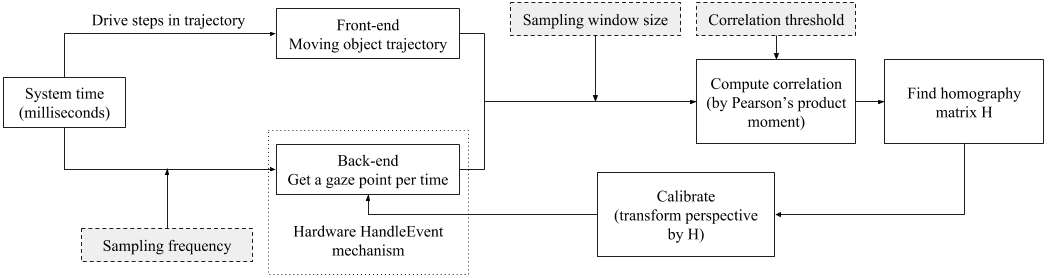
\includegraphics[width=2\columnwidth]{figures/Processing_Pipeline}\\
\caption{The whole processing pipeline in back-end gaze tracking}~\label{fig:figure2}
\end{figure*}
Zhang \textit{et al}. made \textit{SideWays} using off-the-shelf web camera to fulfill instant eye tracking without user calibration \cite{zhang2013sideways}. They took RGB video frame as input, discriminated gaze direction by computing distance between eye centre and inner eye corners for both eyes using image processing in OpenCV, and conducted user studies to validate calibration with tasks of selecting, scrolling and sliding, but their studies showed part of participants reported the tasks are mentally demanding and tiring their eyes. Zhang \textit{et al}. made \textit{GazeHorizon} by a single web camera to navigate content in public displays \cite{zhang2015eye}\cite{zhang2014gazehorizon}, they used computer vision to track the face, extract and process eye images, and computed the horizontal gaze direction based on the PCR method \cite{zhang2013sideways}\cite{zhang2014pupil}, and mapped gaze direction for rate-controlled navigation without prior calibration. However, their gaze navigation cannot be robustly attainable on vertical direction, and subject to head movements.


Pfeuffer \textit{et al}. implemented calibration based on smooth pursuit eye movement \cite{pfeuffer2013pursuit}.smooth pursuit eye movement is a closed-loop system under slight positive feedback \cite{robinson1965mechanics}, continuously adjusting the eye movement according to perceived velocity of moving object being followed, and not a sampled system like saccade. Based on that, Pfeuffer \textit{et al}. computed the correlation using Pearson\textquotesingle s product-moment for the horizontal and vertical gaze position, and fit gaze into projection model homography computation of OpenCV, using RANSAC for outlier elimination with default parameter setting. Vidal \textit{et al}. studied the influence of different parameter settings on pursuit detection performance \cite{vidal2013pursuits}, including number, speed and trajectory of moving objects, and window size and correlation threshold. They also designed and evaluated six pursuit applications, demonstrating pursuit independence of object size, inappropriateness of moving text for reading, and vulnerability of detection performance towards head movements.

Feit \textit{et al}. conducted gaze tracking accuracy and precision data analysis \cite{feit2017toward}, with emphasis on everyday gaze tracking. They statistically studied accuracy (absolute offset) and precision (standard deviation), and based on that computed appropriate target sizes, and optimized the parameters of commonly used filters. 
\section{Method}
I use Tobii eyeX gaze tracker and its C API to implement the back-end gaze tracking, and use Unity3d to design the front-end calibration tasks. I test with my own dedicated gaze, with desktop setup and in undisturbed environment with both daylight and fluorescent lamp. Front-end calibration object is designed as following a seagull that flies in a sinusoidal curvature, and back-end gaze tracking is set as unfiltered.

I pre-define the trajectory of front-end moving object is driven by system-wise time, so that after I stream gaze point in back-end using gaze tracker, I can match gaze points with associated object positions by synchronized system-wise time. Then I compare the similarity between the movement patterns of this two streams by Pearson\textquotesingle s product-moment correlation computation. Once finding the correlation of this two streams lies above pre-defined threshold in certain time intervals, namely the gaze of test subject follows the movement of the object at that time, then I have this two streams within those time intervals as calibration reference, calibrate the following gaze using pinhole projection model and homography matrix in OpenCV with RANSAC outlier elimination in default parameter setting.

The whole processing pipeline is shown in figure 2. Design variables in gaze tracking are sampling frequency, sampling window size and correlation threshold. The necessity to control the sampling frequency is due to inherently unstable gaze point sampling frequency of eye tracker hardware, and choice of both sampling window size and correlation threshold would be a trade-off between calibration speed and accuracy.

\begin{comment}
\subsection{Work Breakdown (comment out)}
Re-implement solutions from Gellersen et al. first, then spend more time in designing calibration tasks. Practically, current implementing pipeline including computing correlation, sampling gaze and calibrating offset using C API of Tobii eye tracker engine,  and designing calibration tasks using Unity3d, then synchronize the gaze pattern from Tobii C API with calibration tasks in Unity3d with timestamp stream of system time in the same computer.
\end{comment}

\begin{comment}
\textit{Implement pipeline}
\begin{itemize}
\item Compute correlation. Compare trajectory of gaze points and moving item, and get quantified correlation index, currently the index is calculated as Pearson\textquotesingle s product-moment.
\item Sample gaze. If judging eyes as following the moving item, then starting or continuing calibration.
\item Model offset calibration. Fit gaze into projection model, may need to identify eye position for it.
\end{itemize}
\textit{Evaluate Calibration}
\begin{itemize}
\item Identify viable design space for item movement with regard to trajectory, speed, item size, etc, with sufficient calibration accuracy and time responsiveness.
\end{itemize}
\textit{Design calibration Tasks}
\begin{itemize}
\item Design 3-5 types of calibration task within or on top on display content.
\item Compare accuracy, time responsiveness and non-intrusiveness of calibration result.
\end{itemize}
\end{comment}

\begin{comment}
\subsection{Main Methods (comment out)}
\textit{Data analysis}\\
It gets involved in both technical implementation and evaluation and design, especially identification of viable design space with sufficient calibration accuracy and speed.

\textit{Field experiment}\\
By conducting field experiment, I collect audience gaze data and also their self-report as "ground-truth" for later calibration accuracy analysis.

\textit{Threats to validity}\\
\textit{Controlled gaze pattern}, audience gaze in field experiment tend to appear more concentrated, compared to the gaze in the wild. Specifically it would threaten sensible gaze sample threshold setting, and viable design space identification for item movement. \textit{Possible improvement} is simulated suitable task for field experiment subjects, making trade-off between ecological validity and technical feasibility.
\end{comment}
% Use a numbered list of references at the end of the article, ordered
% alphabetically by first author, and referenced by numbers in
% brackets~\cite{ethics, Klemmer:2002:WSC:503376.503378,
%   Mather:2000:MUT, Zellweger:2001:FAO:504216.504224}. For papers from
% conference proceedings, include the title of the paper and an
% abbreviated name of the conference (e.g., for Interact 2003
% proceedings, use \textit{Proc. Interact 2003}). Do not include the
% location of the conference or the exact date; do include the page
% numbers if available. See the examples of citations at the end of this
% document. Within this template file, use the \texttt{References} style
% for the text of your citation.

% Your references should be published materials accessible to the
% public.  Internal technical reports may be cited only if they are
% easily accessible (i.e., you provide the address for obtaining the
% report within your citation) and may be obtained by any reader for a
% nominal fee.  Proprietary information may not be cited. Private
% communications should be acknowledged in the main text, not referenced
% (e.g., ``[Robertson, personal communication]'').
\section{Results and Analysis}
According to the figure 2, so far the calibration by transforming perspective using homography matrix part has bugs with OpenCV. In terms of on other parts in the whole pipeline, the front-end object moves at the horizontal speed of 0.5 pixel/millisecond. Comparison between gaze points tracking with known object trajectory is shown in figure 3, 
\begin{figure*}[h!]
  \centering
  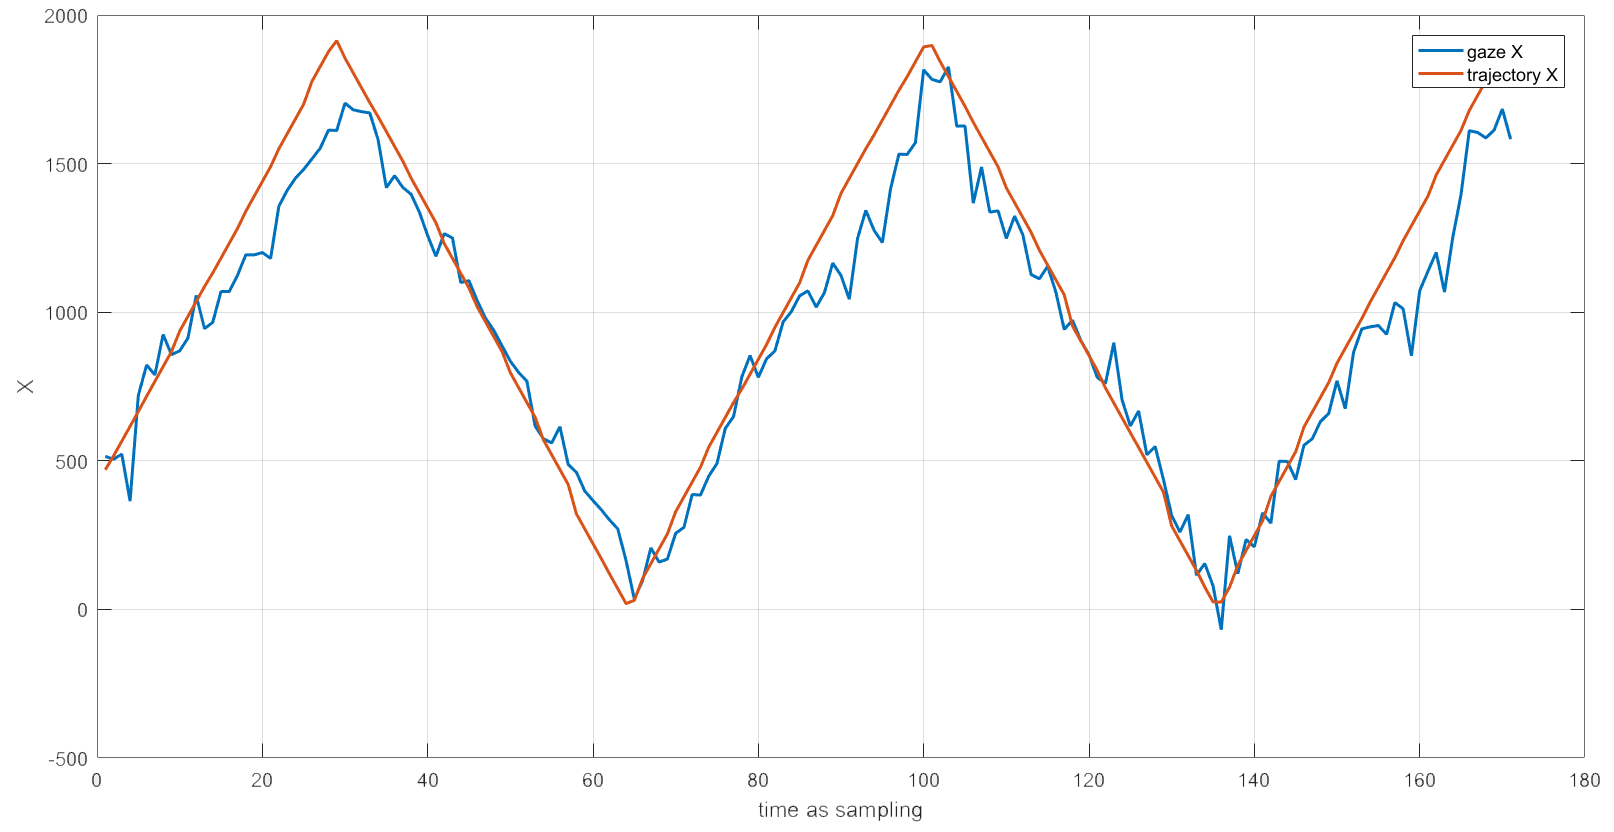
\includegraphics[width=0.65\columnwidth]{figures/Results_X}\space\space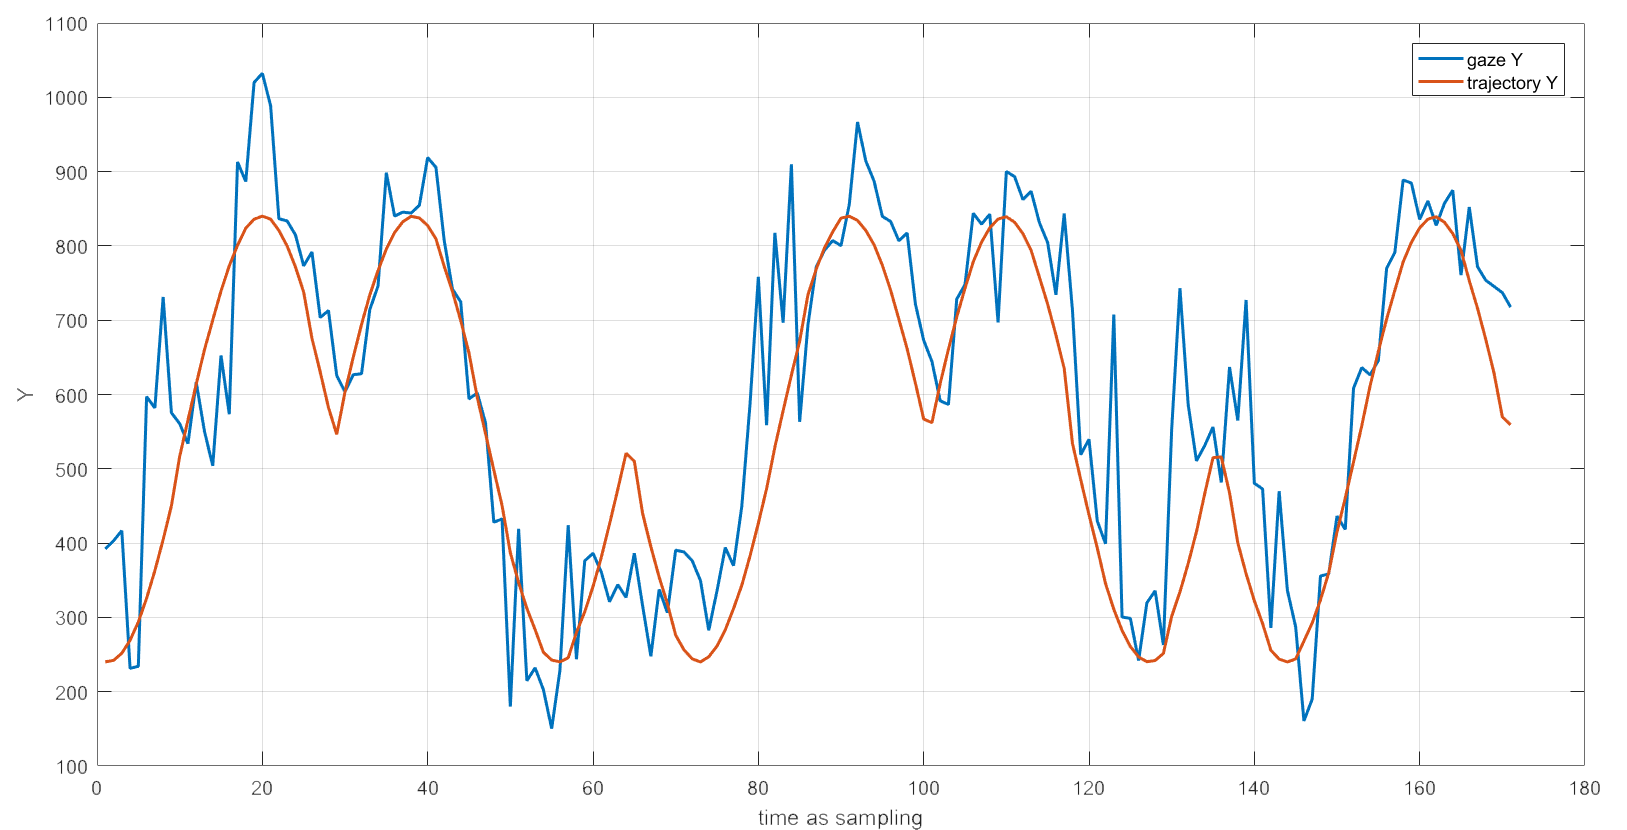
\includegraphics[width=0.66\columnwidth]{figures/Results_Y}\space\space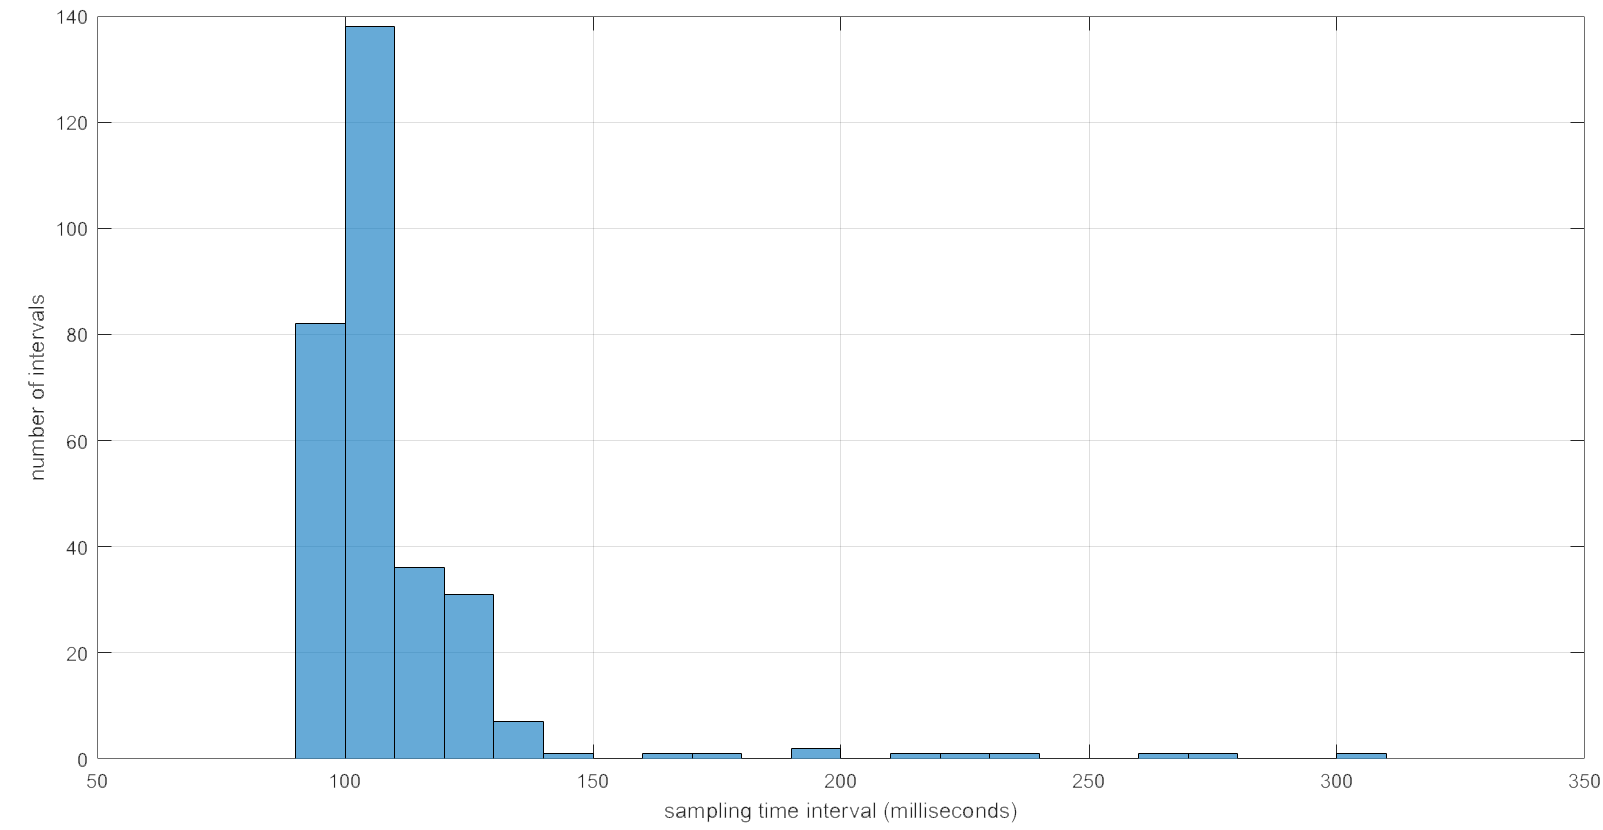
\includegraphics[width=0.64\columnwidth]{figures/sampleFreq}\\
\caption{Gaze tracking before calibration, object moves in periodical back-and-forth sinusoidal curvature: left, X coordinates; middle, Y coordinates (screen width=1920, screen height=1080, window size=4, sampling frequency=10Hz, correlation threshold=0.5); right: sampling time interval distribution in milliseconds}~\label{fig:figure2}
\end{figure*}

\textit{Calibration speed}\\
To find homography matrix to calibrate, it at least needs four pairs of matched gaze points and object trajectory points, with sampling frequency of around 10Hz, in theory a calibration update cycle at least requires 400 ms if the gaze of public display audience follows the moving object trajectory. 

\textit{Moving object trajectory}\\
Due to the ambiguous projection of straight line in 3D space, the moving object trajectory that is as calibration reference can not be straight line under current pinhole projection model and homography matrix computation.
\section{front-end calibration task designs}
To better support getting eligible gaze points following moving object trajectory, and enabling efficient homography matrix calculation, the front-end calibration task designs has the following design objectives, 1) \textit{salient}, moving item attracts visual attention to initiate the calibration, 2) \textit{computational efficient}, using shorter trajectory to calculate more accurate homography matrix, and 3) \textit{non-distractive}, keep the distraction by moving item in the calibration task under sensible level.

I generate the following design candidates in figure 4. 1) moving or swinging items in certain trajectory, and 2) moving point within certain widgets, e.g. columnar timer to count down the display of current content.
\begin{figure}[h!]
  \centering
  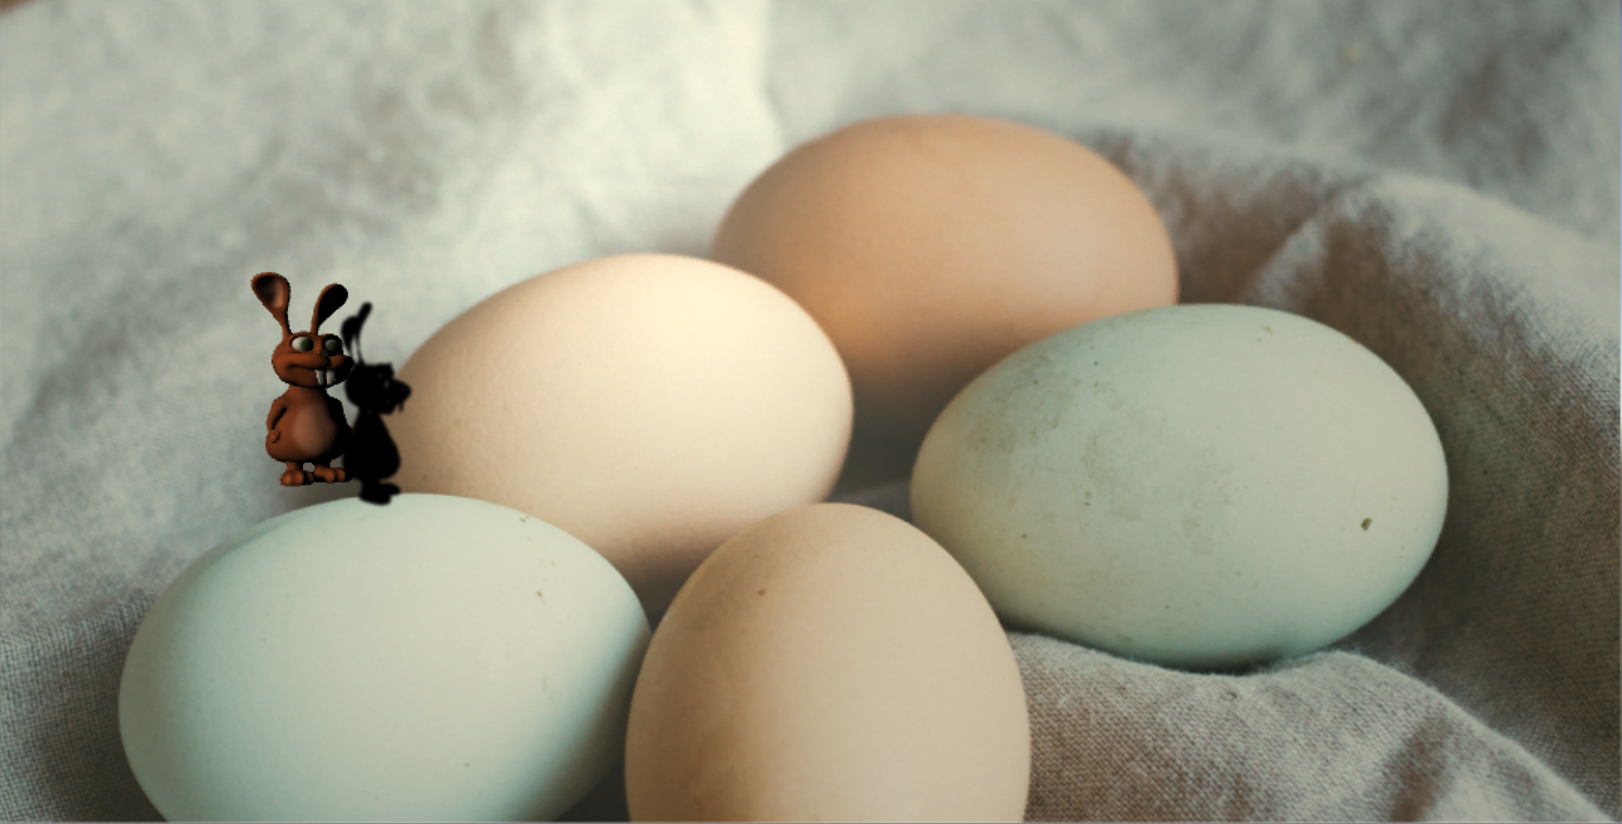
\includegraphics[width=0.47\columnwidth]{figures/EasterAds}\space\space 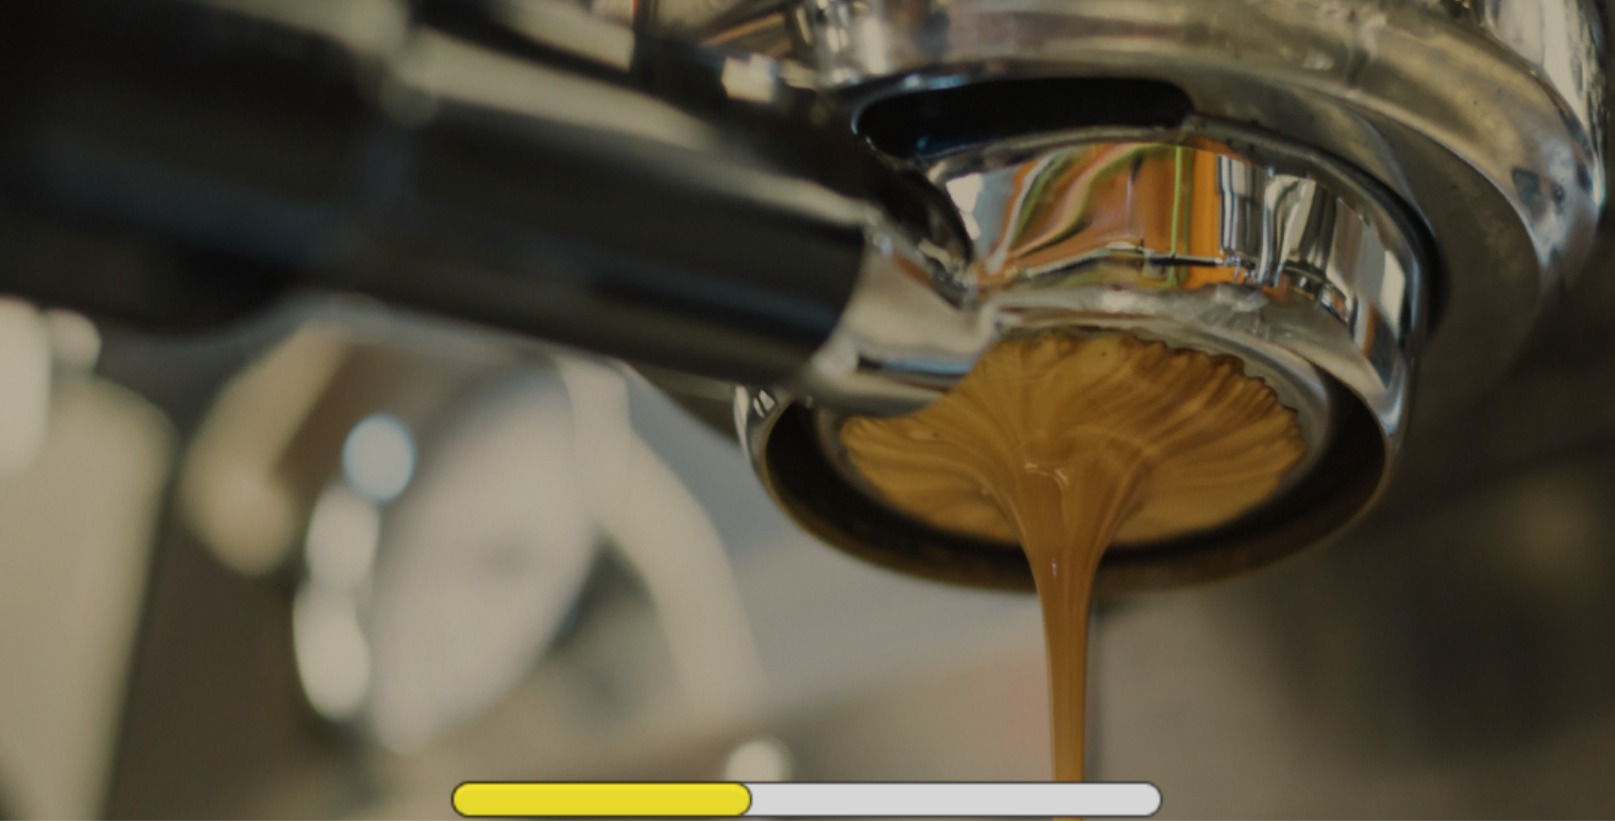
\includegraphics[width=0.47\columnwidth]{figures/CoffeeAds}\\
\caption{Calibration task designs. Left: rabbit moves in the trajectory above eggs; right: bottom timer indicates the time left for displaying current advertisement}~\label{fig:figure2}
\end{figure}

%\section{Acknowledgments}

% Balancing columns in a ref list is a bit of a pain because you
% either use a hack like flushend or balance, or manually insert
% a column break.  http://www.tex.ac.uk/cgi-bin/texfaq2html?label=balance
% multicols doesn't work because we're already in two-column mode,
% and flushend isn't awesome, so I choose balance.  See this
% for more info: http://cs.brown.edu/system/software/latex/doc/balance.pdf
%
% Note that in a perfect world balance wants to be in the first
% column of the last page.
%
% If balance doesn't work for you, you can remove that and
% hard-code a column break into the bbl file right before you
% submit:
%
% http://stackoverflow.com/questions/2149854/how-to-manually-equalize-columns-
% in-an-ieee-paper-if-using-bibtex
%
% Or, just remove \balance and give up on balancing the last page.
%
\balance{}

% BALANCE COLUMNS
\balance{}

% REFERENCES FORMAT
% References must be the same font size as other body text.
\bibliographystyle{SIGCHI-Reference-Format}
\begin{comment}
fix citation problems!
\end{comment}
\bibliography{sample}

\begin{comment}
\section{Appendix}
\subsection{User Research}
\textit{Objectives}\\
User groups statistics of overall ads targeting and audience gaze pattern in the wild, help this paper understand the significance of interpreting audience interest from their gaze data, provide user data on their gaze traits and help identify effective approach of gaze interpretation.Via making personas and scenarios, this paper assumes exemplificative figures and work flow to model their gaze activities and associated interests.

\textit{User Groups Statistics}\\
User study conducted by Florian Alt [] asking 15 people to walk through rooms setting up with digital display and spend as much time there as they wanted. Their pilot data showed people are more engaged with display content when they are standing, indicating by percentage of time shoulders are parallel to display; under optimal environment (less abstraction and more relaxed pace) when people are engaging with ads content, their distance to display is around 1.7 meters, while the distance in the wild is more likely longer.
\begin{table}[h!]
  \centering
  \begin{tabular}{l c c}
    % \toprule
    {\small\textit{Measure}}
    & {\small \textit{Mean}}
    & {\small \textit{Std.dev}} \\
    \midrule
    shoulders parallel time (\%) & 69.5 & 17.2 \\
      shoulders parallel time while walking (\%) & 46.3 & 16.1 \\
    shoulders parallel time while standing (\%) & 82.0 & 18.6 \\
    mean distance from display (m) & 1.7 & .41 \\
    % \bottomrule
  \end{tabular}
  \caption{User study data}~\label{tab:table1}
\end{table}
This paper conducts informal field observation in Kamppi, finding most of people who gaze at ads in public displays are keeping walking, the time they spend gazing are around 3 seconds, and engagement at the moment of their leaving indicating by their head-turning degree and gaze fixations can strongly show their interest on ads.
\end{comment}

\begin{comment}
\subsection{Gaze Tracking Pilot Setup Walk-through (comment out)}
To experience the feasibility of the whole research pipeline, I conduct pilot test with myself using Tobii eye tracker and desktop setup. I directly log output gaze data stream from Tobii eye tracker API, and read them into Matlab to process. I set centre and corner reference points in full-screen, and record gaze points coordinates when audience looks at these points. Then clustering gaze point groups into associated centre gaze points using k-means, and compare centre gaze points with reference points (figure 1). There's difference between this two, but temporarily I haven't calibrated further. Just superimpose gaze points with ads in the same coordinate. Based on empirical gaze data, I divide $1920\times 1080$ ads into $30\times 30$ grids, and generate heat-map according to number of gaze points lie in associated area (figure 2). Area of interest is indicated as yellow areas.
\begin{figure}[h!]
  \centering
  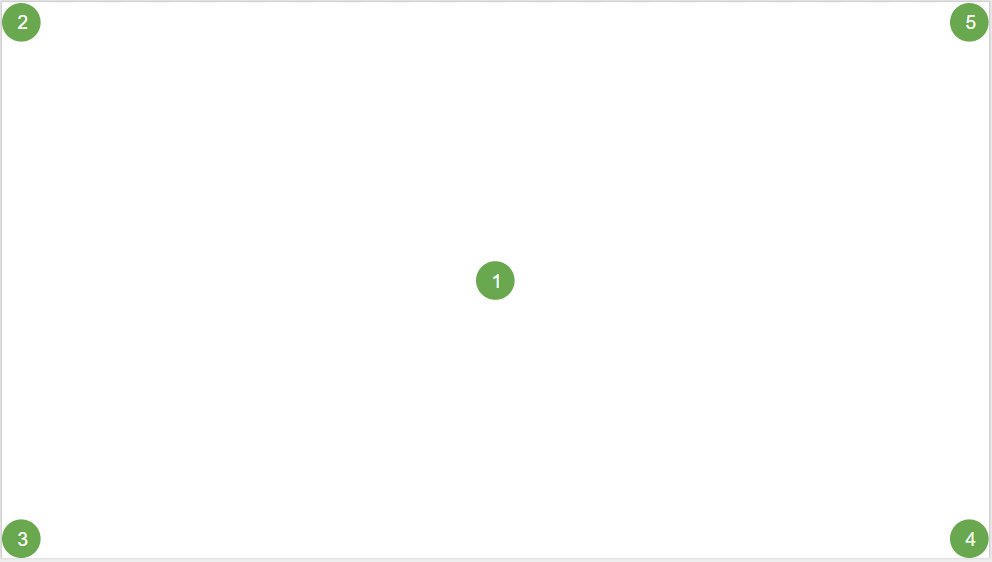
\includegraphics[width=0.4\columnwidth]{figures/calibrate_original}\space\space 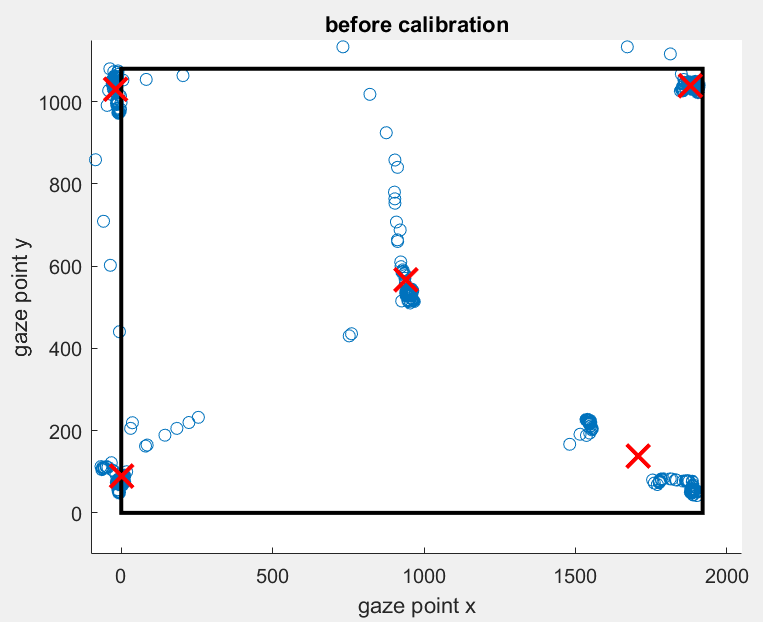
\includegraphics[width=0.4\columnwidth]{figures/calibrate_before}\\
  \caption{Calibrate gaze points}~\label{fig:figure2}
\end{figure}
\begin{figure}[h!]
  \centering
  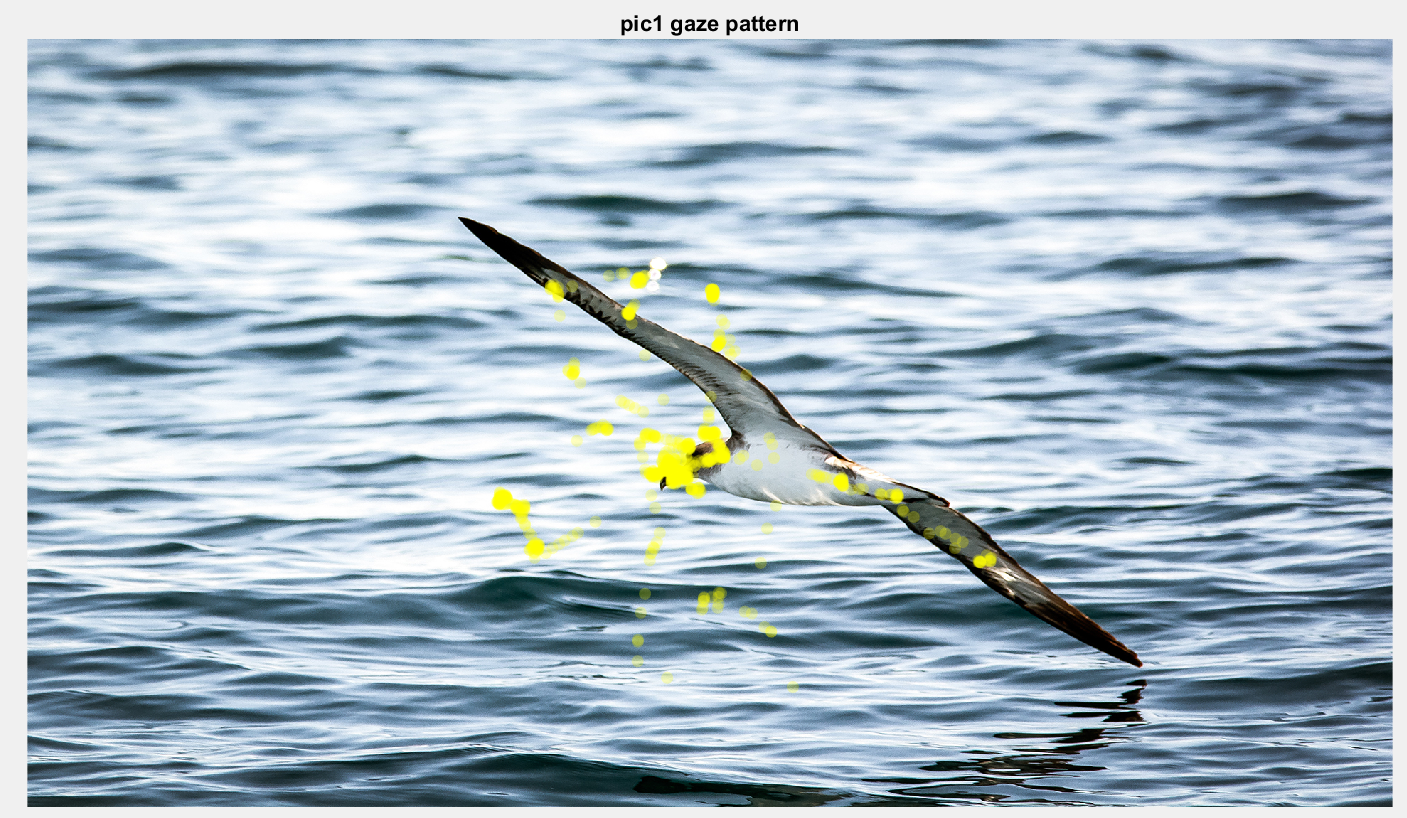
\includegraphics[width=0.4\columnwidth]{figures/pic1_gaze_pattern}\space\space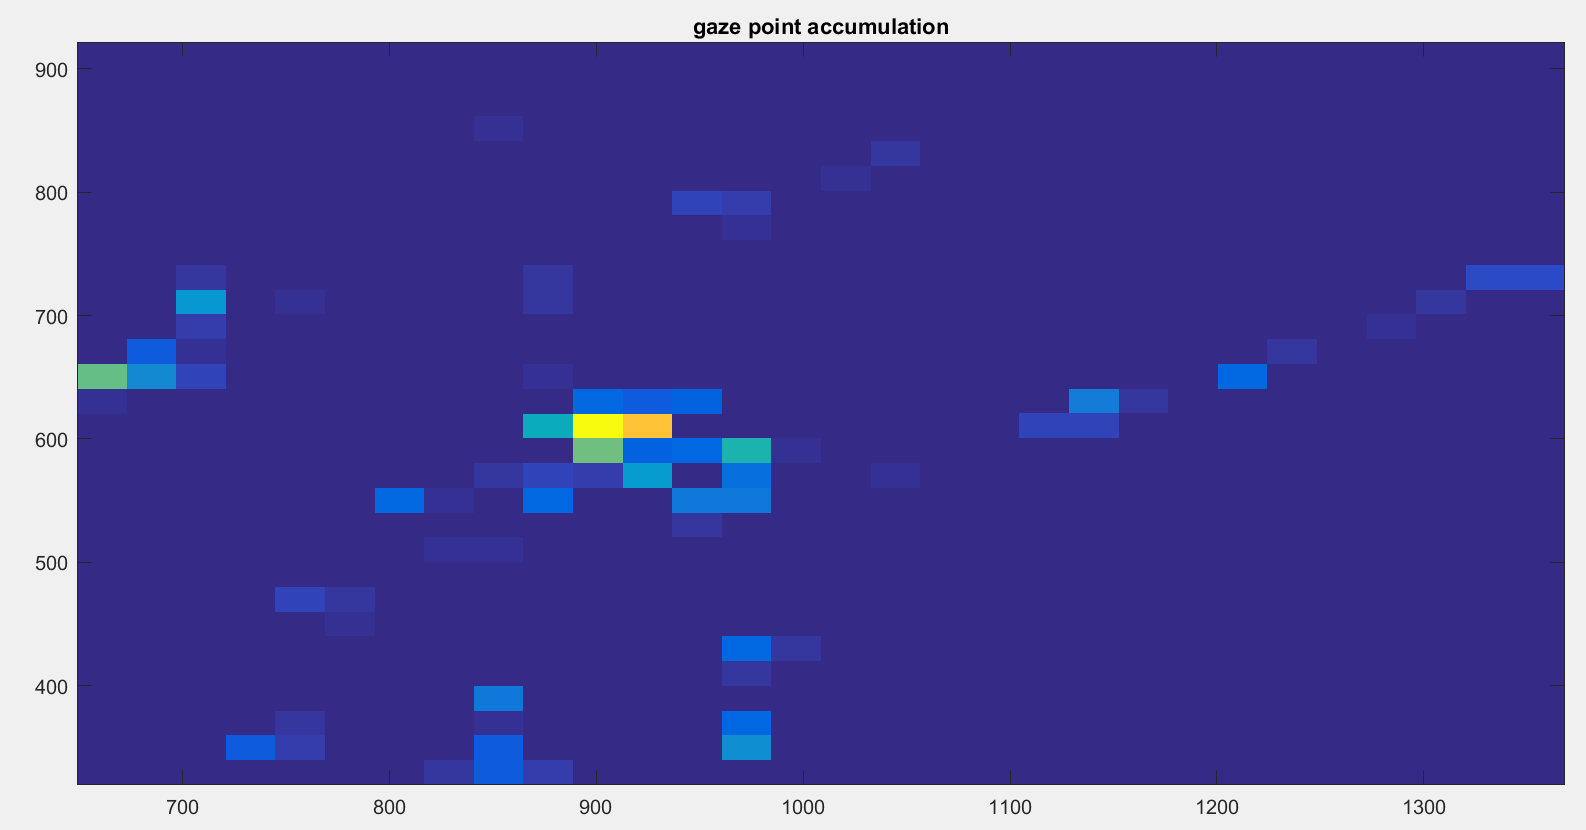
\includegraphics[width=0.45\columnwidth]{figures/heatMap}\\
  \caption{Gaze points on picture}~\label{fig:figure2}
\end{figure}
\end{comment}

\begin{comment}
\subsection{Naive Calibration Pilot}
\textit{Pipeline}\\
Streaming gaze points from Tobii eye tracker API, using a window to sample gaze points (window length = 50), computing correlation index within a window. If correlation indices of three consecutive windows are above predefined threshold, using gaze points of this three windows to compute offset against moving object trajectory; once correlation index is below the threshold before finding three satisfied consecutive windows, restarting accumulating consecutive windows.
\begin{figure}[h!]
  \centering
  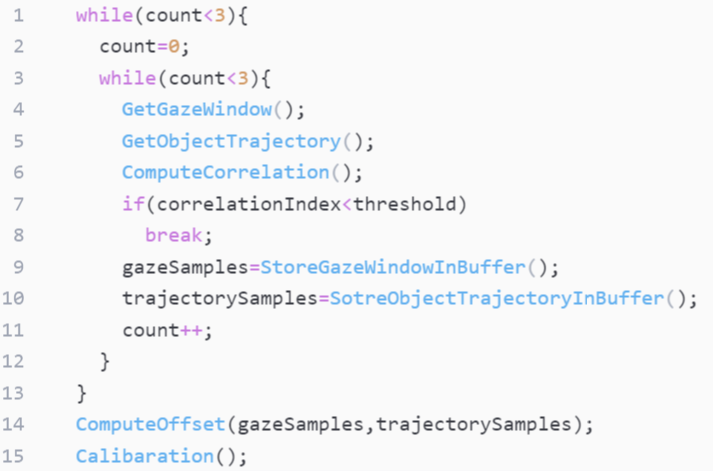
\includegraphics[width=1\columnwidth]{figures/Pipeline}\\
  \caption{Pipeline pseudocode}~\label{fig:figure2}
\end{figure}\\
\textit{Compute Correlation Index}\\
Pearson\textquotesingle s product-moment (see equation (1)) for the horizontal and vertical gaze position.
\begin{align}
correlation=\frac{\sum(X-\overline{X})(Y-\overline{Y})}{(\sqrt{\sum^{n}_{i=1}(X_i-\overline{X})^{2}})(\sqrt{\sum^{n}_{i=1}(Y_i-\overline{Y})^{2}})}
\end{align}

\textit{Compute Offset}\\
Calculating Euclidean distance between gaze point and associated point in object trajectory on both horizontal and vertical dimensions, and then calculate mean distance as offset respectively.
\begin{figure}[h!]
  \centering
  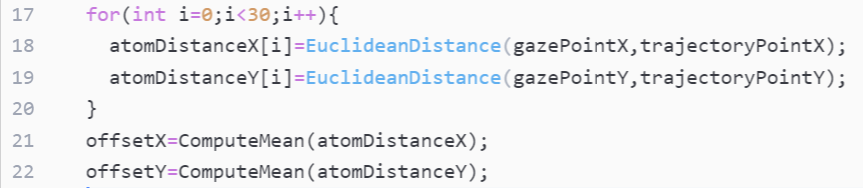
\includegraphics[width=1\columnwidth]{figures/Offset}\\
  \caption{Compute offset pseudocode}~\label{fig:figure2}
\end{figure}\\
\textit{Calibration}\\
Simply plus or minus streaming of gaze coordinates from eye tracker with 2D offset vector.

\textit{Sample Object Trajectory}\\
A sphere moves in ping-pong manner horizontally.

\textit{Current Progress}\\
Finished the designs of overall simplified logic, sub-functions and synchronizing backstage gaze tracking with upfront calibration task design. Working on piloting sensible data, and then upgrading calibration module and task designs.
\end{comment}

\begin{comment}
\subsection{Data Analysis (comment out)}

\textit{Objectives}\\
Evaluating the accuracy and time-responsiveness of calibration, also comparing calibration effect of different calibration task designs, and generalizing calibration effect of several design variable settings in calibration task design.

\textit{Resolution Steps}\\
Collect gaze tracking data and 'ground-truth' from user testing (minimum one person).\\
Clean and pre-process collected data.\\
Evaluate calibration accuracy (?) and time-responsiveness.\\
Compare calibration accuracy and time-responsiveness under different calibration task designs.\\
Set different design variables in calibration tasks as independent variable respectively, generalize calibration effect of these design variables.
\end{comment}

\end{document}

%%% Local Variables:
%%% mode: latex
%%% TeX-master: t
%%% End:
